\documentclass[final]{beamer}

%\usepackage{microtype}

\usepackage[orientation=landscape,size=a0,scale=1.7]{beamerposter}
\usepackage{calc}
\usepackage{commath}
\usepackage[no-math]{fontspec}
\usepackage{mathspec}
\usepackage{nag}
\usepackage{siunitx}
\usepackage{tcolorbox}

\tcbuselibrary{raster}

\setmainfont{Noto Serif}
\setsansfont{Open Sans}
\usefonttheme[onlymath]{serif}
\setmathfont(Digits,Latin,Greek){Noto Serif}

\useinnertheme{circles}
\setbeamercolor{itemize item}{fg=black}
\setlength{\leftmargini}{.7\baselineskip}

\setbeamercolor{block title}{fg=black}
\setbeamerfont{block title}{series=\bfseries,size=\normalsize}

%gets rid of navigation symbols
\setbeamertemplate{navigation symbols}{}

\tcbset{
    boxsep=5mm, titlerule=0mm,
    colback=white, colframe=black, arc=0mm,
    fonttitle=\bfseries,
    coltitle=black, colbacktitle=white,
    halign title=center, halign=flush left
}



\title{A Spiking Independent Accumulator Model for\\Winner-Take-All Computation}
\author{Jan Gosmann, Aaron R. Voelker, Chris Eliasmith \{jgosmann, avoelke, celiasmith\}@uwaterloo.ca}
\institute{Centre for Theoretical Neuroscience, University of Waterloo <http://ctn.uwaterloo.ca>}

\begin{document}
\begin{frame}[t]
    \begin{columns}
        \begin{column}{129mm}
            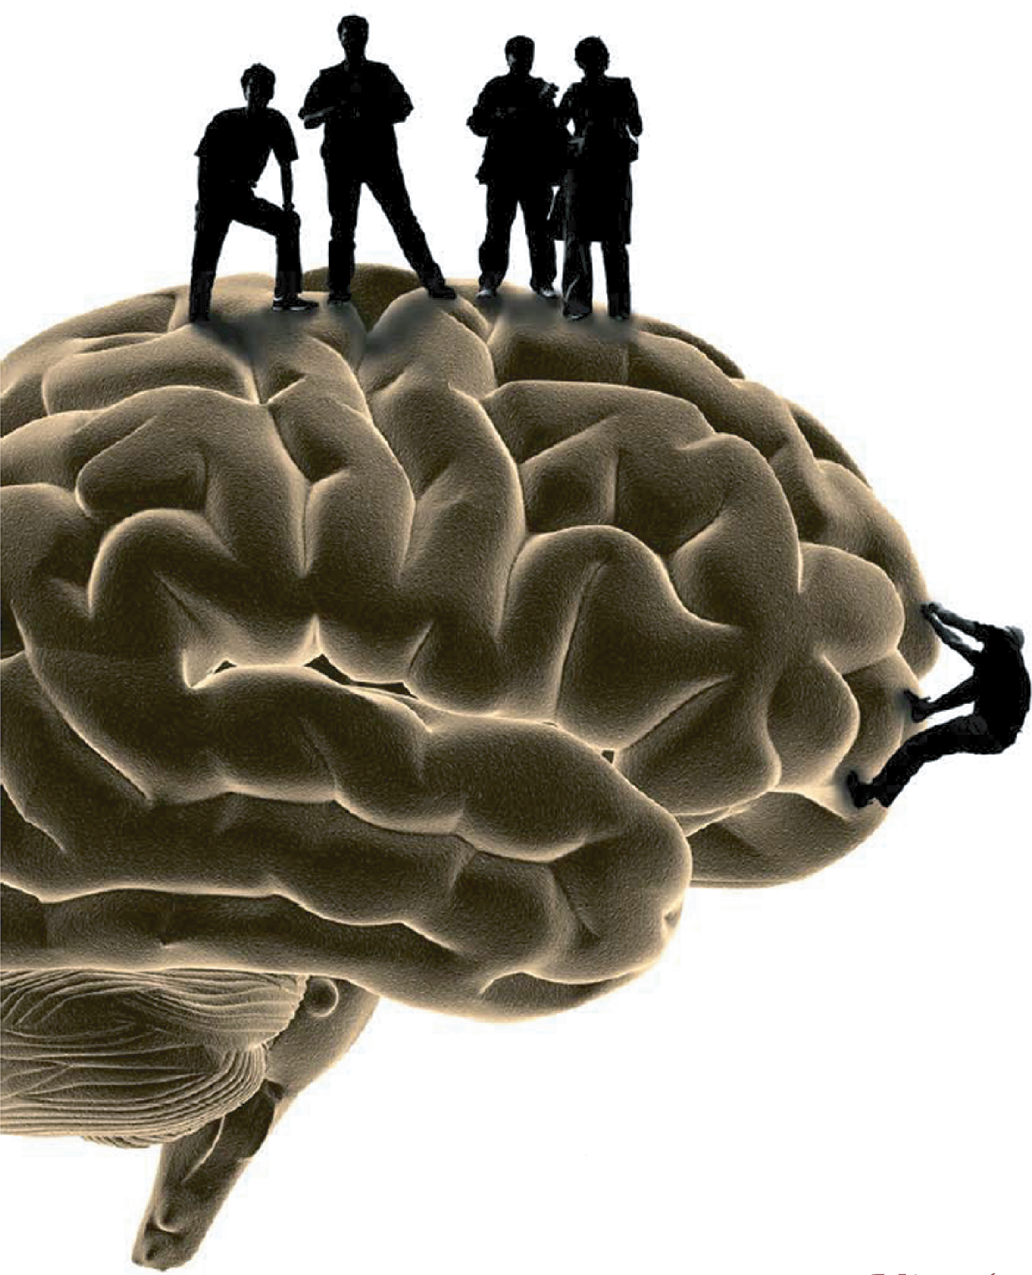
\includegraphics[width=128mm]{People_brain}
        \end{column}
        \begin{column}{\paperwidth-339mm}
            \begin{center}
                {\huge\inserttitle\par}

                \vspace*{10mm}
                \insertauthor\par\insertinstitute%
            \end{center}
        \end{column}
        \begin{column}{190mm}
            \centering
            \raisebox{-0.5\height}{
\includegraphics[trim=96.65 0 0 0,width=102.8mm]{UniversityOfWaterloo_logo_vert_cmyk}}\hfill
            \raisebox{-0.5\height}{
\includegraphics[width=86.8mm]{CTN_logo}}\\
            
\includegraphics[width=187.7mm]{cnrg_logo}
        \end{column}
        \begin{column}{20mm}
        \end{column}
    \end{columns}
    \vspace*{20mm}

    \begin{tcbraster}[raster columns=4, raster column skip=10mm, raster row skip=10mm, raster equal height=rows, raster force size=false]
        \begin{tcolorbox}[title=Motivation, add to width=-2cm]
            \begin{itemize}
                \item Investigate WTA mechanisms in the context of neurally plausible cognitive modelling
                \item Implement using spiking neurons
                \item Explore the effect of noisy inputs on stable decision making
                \item Allow for integration into larger scale networks
            \end{itemize}
        \end{tcolorbox}
        \begin{tcolorbox}[title=Neural Engineering Framework, add to width=5cm]
            \begin{itemize}
                \item \emph{Representation} in spiking neurons defined by encoding
                        $a_i(t) = G_i\left[a_i e_i x(t) + J_i^{\mathrm{bias}} \right]$
                        and decoding
                        $\hat{x}(t) = \sum_i d_i \left[(a_i * h)(t) \right]$
                \item \emph{Transformation} by decoding weights $d_i$ minimizing $E_{f(x)} = \abs{f(x) - \hat{x}}$
                \item \emph{Dynamics} by recurrent transformation
                    \begin{equation*}
                        \frac{\partial x}{\partial t} = g(x) \quad\Rightarrow\quad f(x) = \tau_s g(x) + x
                    \end{equation*}
            \end{itemize}
        \end{tcolorbox}
        \begin{tcolorbox}[title=Benchmarks, add to width=-3cm]
            \begin{itemize}
                \item Ability to provide a clear output (single output above \num{0.15}, stable over at least \SI{1}{\second})
                \item Correctness (output corresponds to strongest input)
                \item Time required to reach a decision
                \item Transient outputs before final decision is reached
            \end{itemize}
        \end{tcolorbox}
        \begin{tcolorbox}[title=Conclusions, add to width=0cm]
            \begin{itemize}
                \item The two WTA mechanisms are best suited for different purposes
                \item LCA network:
                    \begin{itemize}
                        \item Reacts more quickly
                        \item If stable decision is reached, it will be correct
                        \item Output can be unstable in noisy conditions
                    \end{itemize}
                    \item IA network: will eventually give a stable output, but it might not be the correct one
            \end{itemize}
        \end{tcolorbox}
        \begin{tcolorbox}[raster multicolumn=4,title={Leaky, Competing Accumulators (LCA)},halign title=left]
            \begin{minipage}[c][6in]{20cm}
                \vfill
                \vfill
                \begin{align*}
                    \frac{{\partial x}_i}{\partial t} &= \left(\rho_i - kx_i - \beta \sum_{j \neq i} x_j\right) \frac{1}{\tau},\\
                    x_i &\ge 0
                \end{align*}
                \vfill
                {\tiny Usher, M., \& McClelland, J.~L. (2001). The time course of perceptual choice: THe leaky, competing accumulator model. \textit{Psychological Review}, 108(3), 550--592.\par}
            \end{minipage}
            \hfill
            \raisebox{-0.5\height}{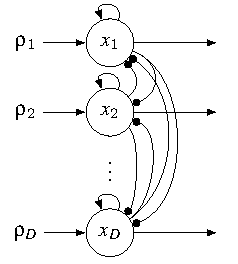
\includegraphics[scale=2.9]{lca-sketch}}
            \hfill
            \raisebox{-0.5\height}{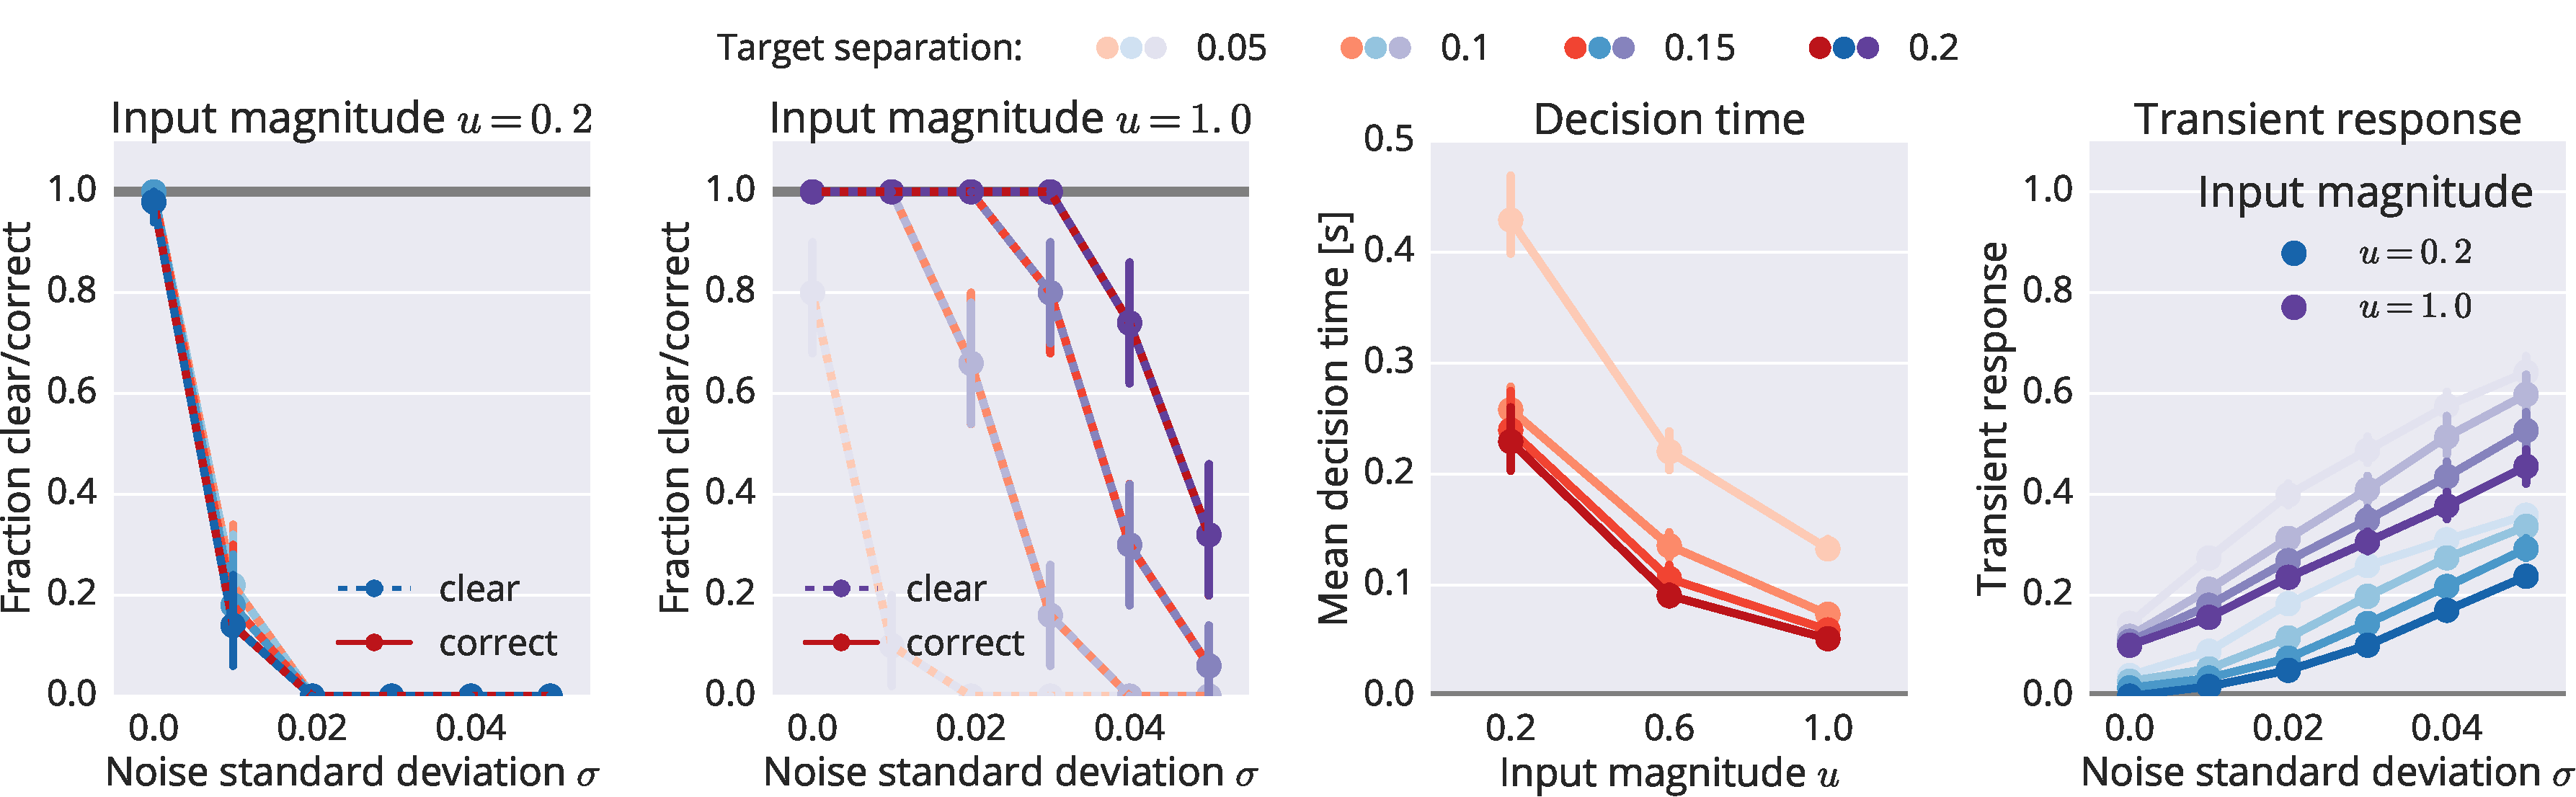
\includegraphics[trim=0 0 0 80]{lca}}
        \end{tcolorbox}
        \begin{tcolorbox}[raster multicolumn=4,title=Independent Accumulators,halign title=left]
            \begin{minipage}[c]{20cm}
                \begin{align*}
                    \bar{x}_i &:= \Theta(x_i - \vartheta),\\
                    \frac{{\partial x}_i}{\partial t} &= \rho_i \frac{1}{\tau_1} + \left( 
            \bar{x}_i - \bar{\beta} \sum_{j \neq i} \bar{x}_j \right) \frac{1}{\tau_2},\\
                    \quad x_i &\ge 0
                \end{align*}
            \end{minipage}
            \hfill
            \raisebox{-0.5\height}{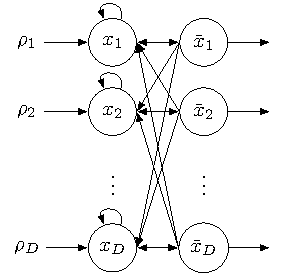
\includegraphics[scale=2.9]{ia-sketch}}
            \hfill
            \raisebox{-0.5\height}{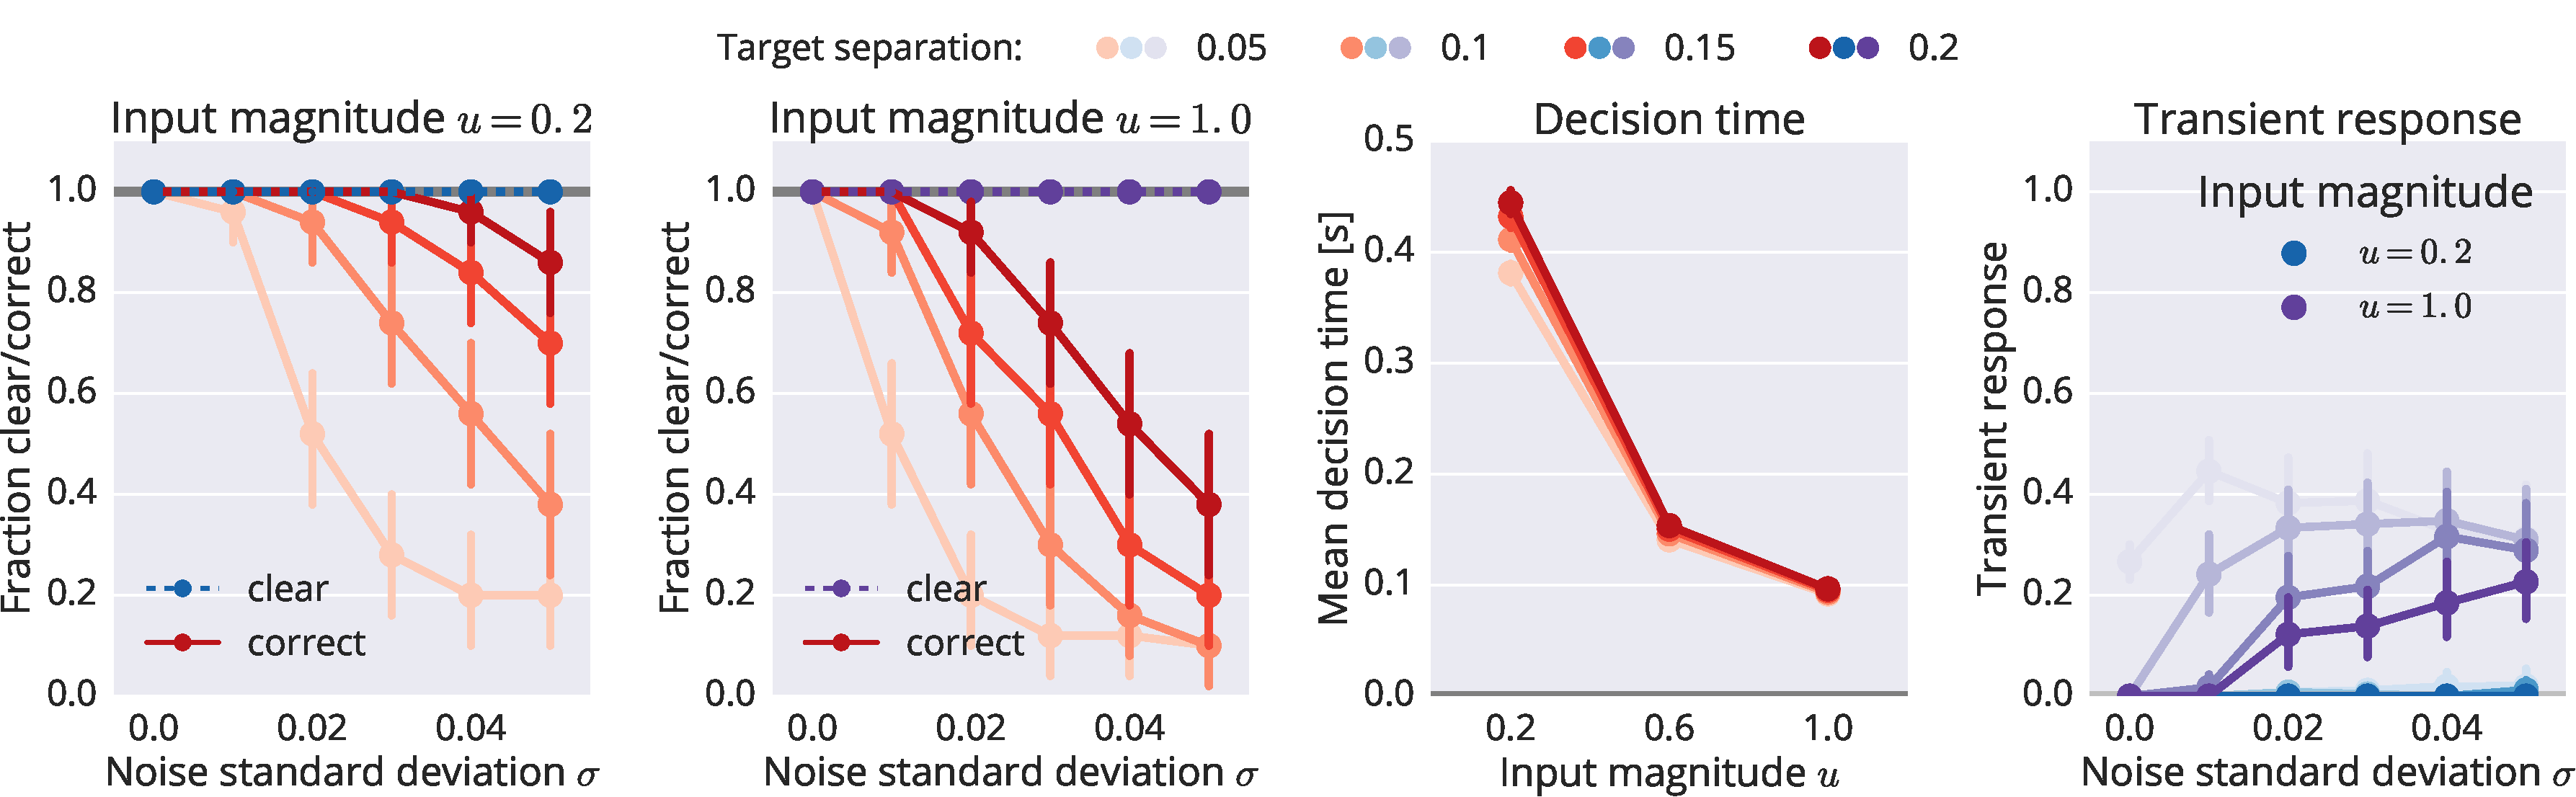
\includegraphics[trim=0 0 0 80]{ia}}
        \end{tcolorbox}
    \end{tcbraster}

\end{frame}

\end{document}
